\newpage
\section{Auswertung}
\label{sec:Auswertung}
\subsection{Verstärkung eines gestörten Sinus-Signales}
\label{sec:Auswertung1}
%Der erste Teil der verwendeten Maschine, der Funktionsgenerator, hat einen Ausgang für Spannung, 
%die in Amplitude, Spannungsform und Frequenz angepasst werden kann, und einen Ausgang, 
%der parallel zum ersten Ausgang die gleiche Spannungsform und Frequenz bei konstanter Amplitude liefert.
Der Effektivwert bei Sinus-förmiger Wechselspannung ist an beiden Ausgängen \SI{4.63}{\volt}, die Frequenz $f$ beträgt $\SI{1}{\kilo\hertz}$.
Mit $U_\text{eff}=\sqrt{2}U_0$ für Sinusschwingungen ergibt sich eine Amplitude von etwa \SI{6.55}{\volt}.
%Weiter wird das Messsignal über einen Verstärker verstärkt und mithilfe eines Bandpasses gefiltert, während das Referenzsignal in einen Phasenwandler geleitet wird.
%Beide Signale werden anschließend in dem Lock-In-Detektor gemischt und
\begin{table}
	\centering
	\begin{tabular}{c S[table-format=1.2]S[table-format=1.2]}
	\toprule
	{Phase}&\multicolumn{2}{c}{Ausgangsspannung $U_0$/[V]}\\
	&{ohne Störung}&{mit Störung}\\
	\midrule
		0°		&-6.00	&-6.00\\
		45°		&-4.00	&-4.00\\
		90°		& 0.20	& 0.50\\
		120°	& 2.62	& 3.00\\
		135°	& 4.25	& 4.50\\
		180°	& 5.81	& 6.00\\
		225°	& 3.95	& 3.50\\
		270°	& 0.20	&-0.50\\
		315°	&-4.17	&-4.50\\
		360°	&-5.83	&-5.50\\
	\bottomrule
	\end{tabular}
	\caption{Ausgangsspannung des gegebenen Signals.}
	\label{tab:spannung}
\end{table}
Die Spannungen, die den Tiefpass und damit den gesamten Lock-In-Verstärker verlassen, sind in Tabelle \ref{tab:spannung} aufgetragen. 
Die angegebene Phase ist die eingestellte Phase des Phasenschiebers.
Diese Spannungen werden in Diagramm \ref{diag:spannung} gegen die eingestellte Phase aufgetragen; 
es zeigt sich, dass die Beziehung \eqref{cosinus_ausgangsspannung} durch die Datenpunkte verifiziert wird, es aber zu einem festen Phasenversatz $\alpha$ von $\alpha=180°$ kommt.
Dies ist nicht darauf zurückzuführen, dass das hier verwandte Referenzsignal nicht normiert-rechteckförmig, sondern sinusförmig ist, 
aber eventuell darauf, dass die Ausgänge des Funktionsgenerators und die Bauteile des Verstärkers einen permanenten Phasenversatz aufweisen bzw. die Leitungen einen Versatz bewirken.
\begin{figure}[htb]
	\centering
	\begin{subfigure}{0.49\textwidth}
		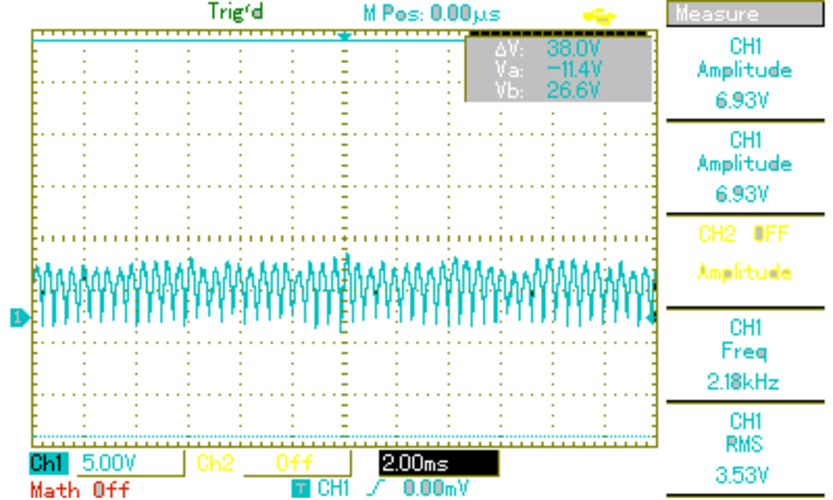
\includegraphics[width=\textwidth]{Bilder/MAP002.pdf}
	\end{subfigure}
	\begin{subfigure}{0.49\textwidth}
		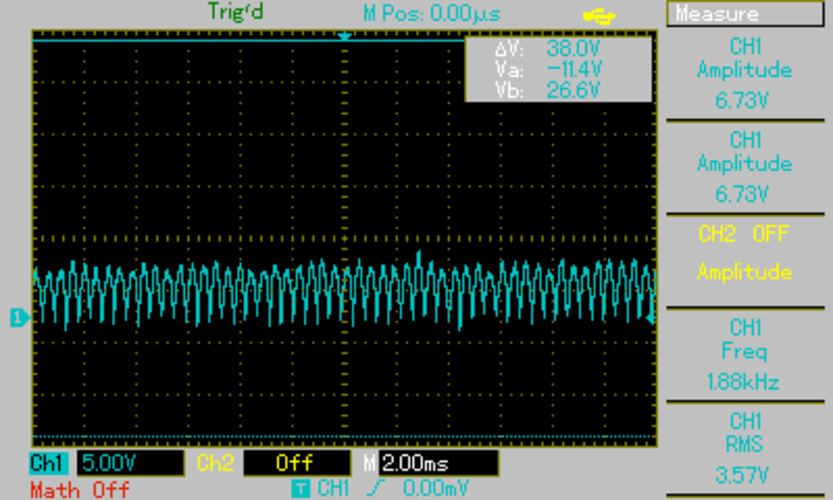
\includegraphics[width=\textwidth]{Bilder/MAP003.pdf}
	\end{subfigure}
	\caption{Fotos des Oszillators: das Signal mit Störungen zu zwei verschiedenen Zeiten. \cite{gimp}}
	\label{fig:stoerung}
\end{figure}
Die Abbildung \ref{fig:stoerung} zeigt das Sinus-förmige Signal mit der überlagerten Störung. 
Trotz der Abweichungen vom idealen Signal werden die Werte der Messung ohne Störung sehr gut angenähert.
\begin{figure}[hp]
	\centering
	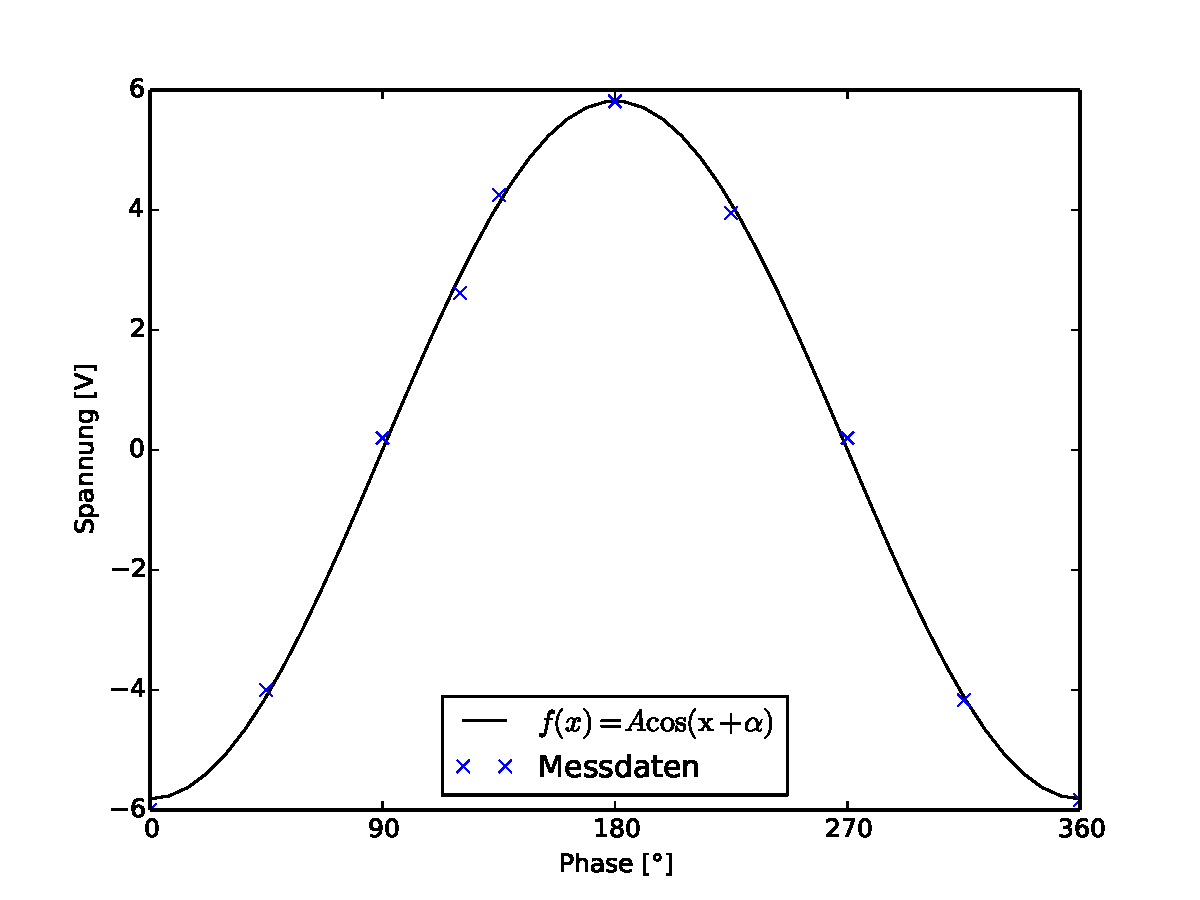
\includegraphics[width=0.8\textwidth]{Bilder/AusgangSpannung.pdf}
	\caption{Ausgangsspannung des Lock-In-Verstärkers bei Sinus-förmigen Eingang mit $U = \SI{4.63}{\volt}$ und $f = \SI{300}{\hertz}$.}
	\label{diag:spannung}
\end{figure}

\begin{figure}[hp]
	\centering
	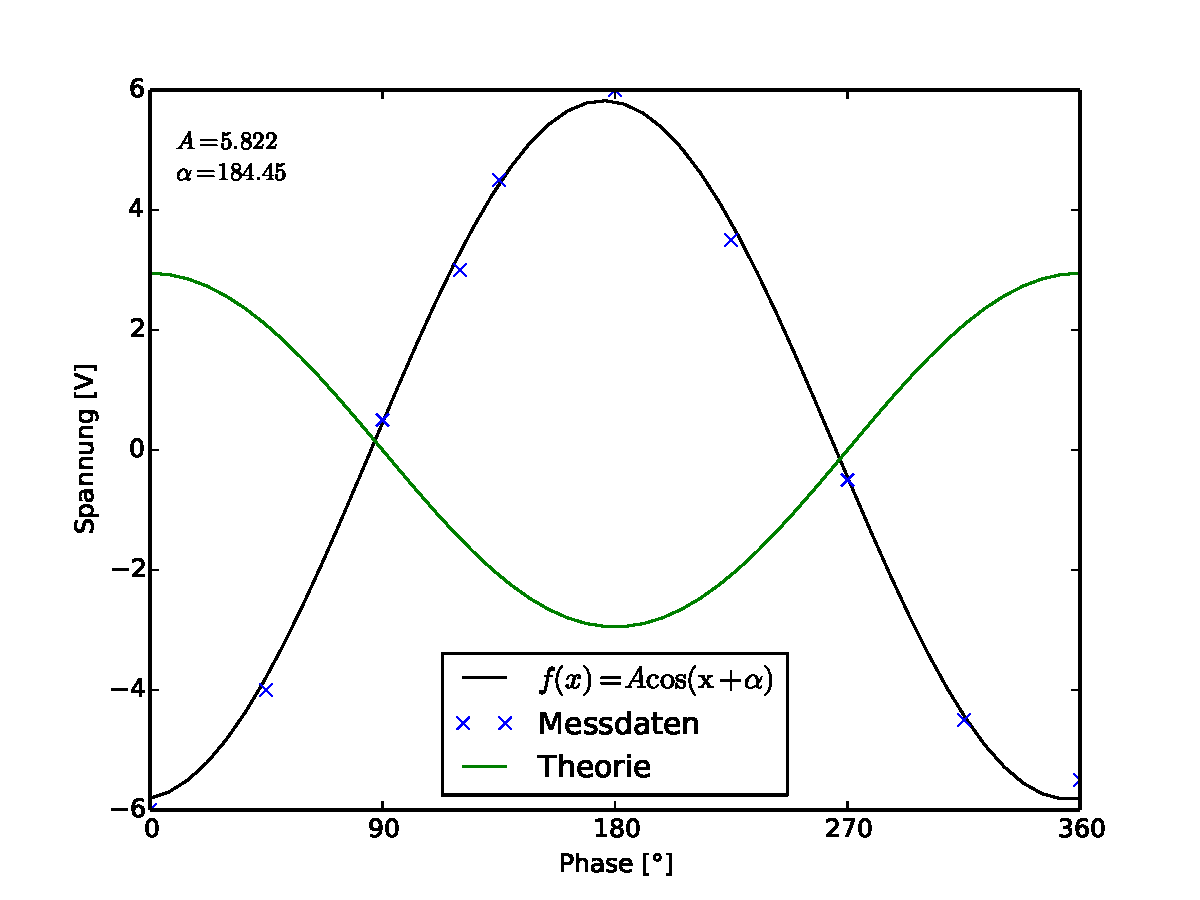
\includegraphics[width=0.8\textwidth]{Bilder/AusgangStoerung.pdf}
	\caption{Ausgangsspannung des Lock-In-Verstärkers bei gestörtem Signal.}
	\label{diag:stoerung}
\end{figure}


\subsection{Verstärkung des LED-Signales}
\begin{table}
	\centering
	\begin{tabular}{c S[table-format=1.2] l c}
	\toprule
	{Abstand a}&{Ausgangsspannung $U_0$}&\multicolumn{2}{c}{Gesamt-Verstärkung}\\
	{$[\si{\meter}]$}&{$[\si{\volt}]$}&{absolut}&{relativ}\\
	\midrule
		0.02&	-5 		& $400\cdot5$ 	 & 1\\
		0.05&	-1 		& $400\cdot5$ 	 & 1\\
		0.08&	-0.5 	& $400\cdot5$ 	 & 1\\
		0.11&	-2 		& $400\cdot50$ 	 & 10\\
		0.14&	-1 		& $400\cdot50$	 & 10\\
		0.17&	-0.9 	& $400\cdot50$	 & 10\\
		0.20&	-6.0	& $400\cdot500$	 & 100\\
		0.23&	-4.5 	& $400\cdot500$	 & 100\\
		0.26&	-3.5 	& $400\cdot500$	 & 100\\
		0.29&	-2.5 	& $400\cdot500$	 & 100\\
		0.39&	-1.0 	& $400\cdot500$	 & 100\\
		0.49&	-0.7 	& $400\cdot500$	 & 100\\
		0.59&	-0.5 	& $400\cdot500$	 & 100\\
		0.69&	-0.3 	& $400\cdot500$	 & 100\\
		0.79&	-0.25 	& $400\cdot500$	 & 100\\
		0.99&	-0.12 	& $400\cdot500$	 & 100\\
		1.19&	-0.1 	& $400\cdot500$	 & 100\\
	\bottomrule
	\end{tabular}
	\caption{Ausgangsspannung bei der Messung des LED-Lichtes.}
	\label{tab:led}
\end{table}
\begin{figure}[hbp]
	\centering
	\begin{subfigure}{0.8\textwidth}
		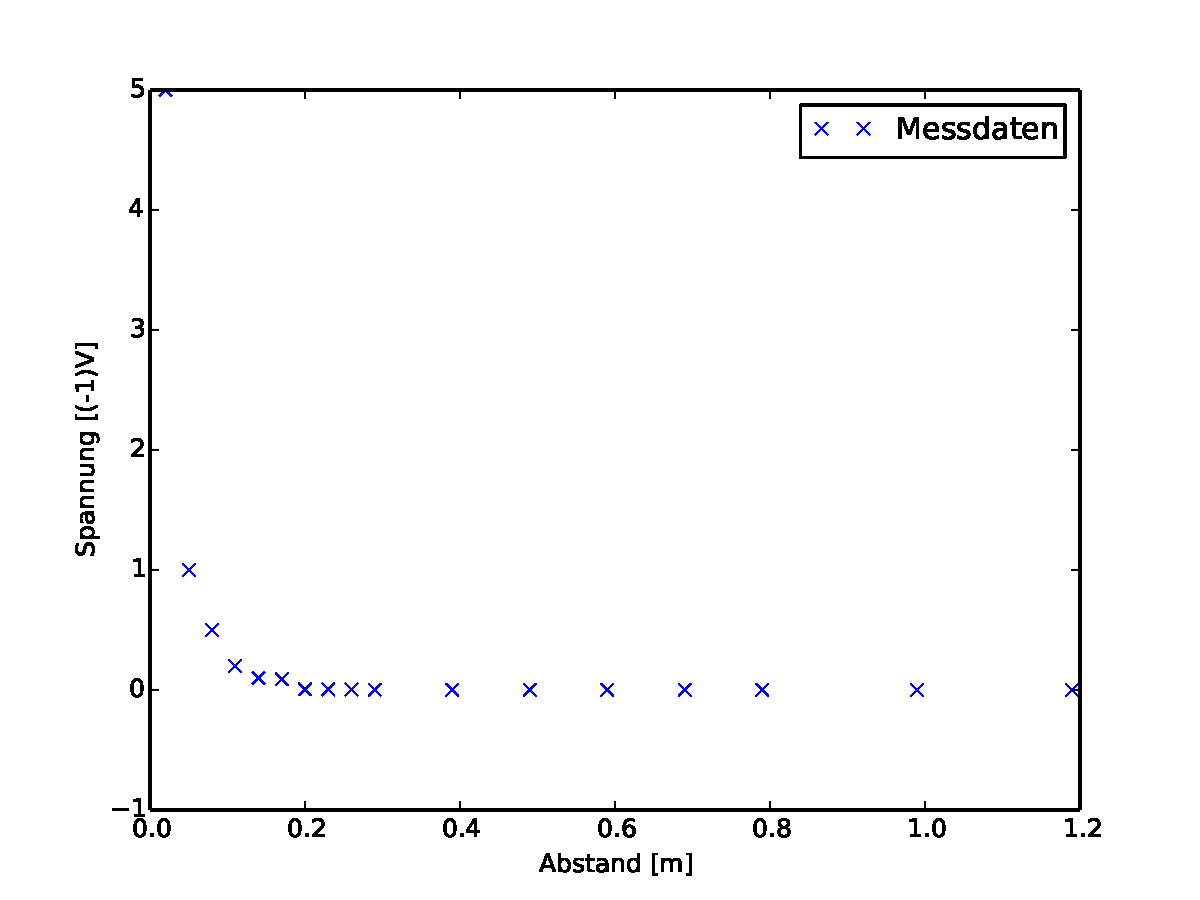
\includegraphics[width=\textwidth]{Bilder/LED.pdf}
		\caption{Lineare Skalierung.}
	\end{subfigure}
	\begin{subfigure}{0.8\textwidth}
		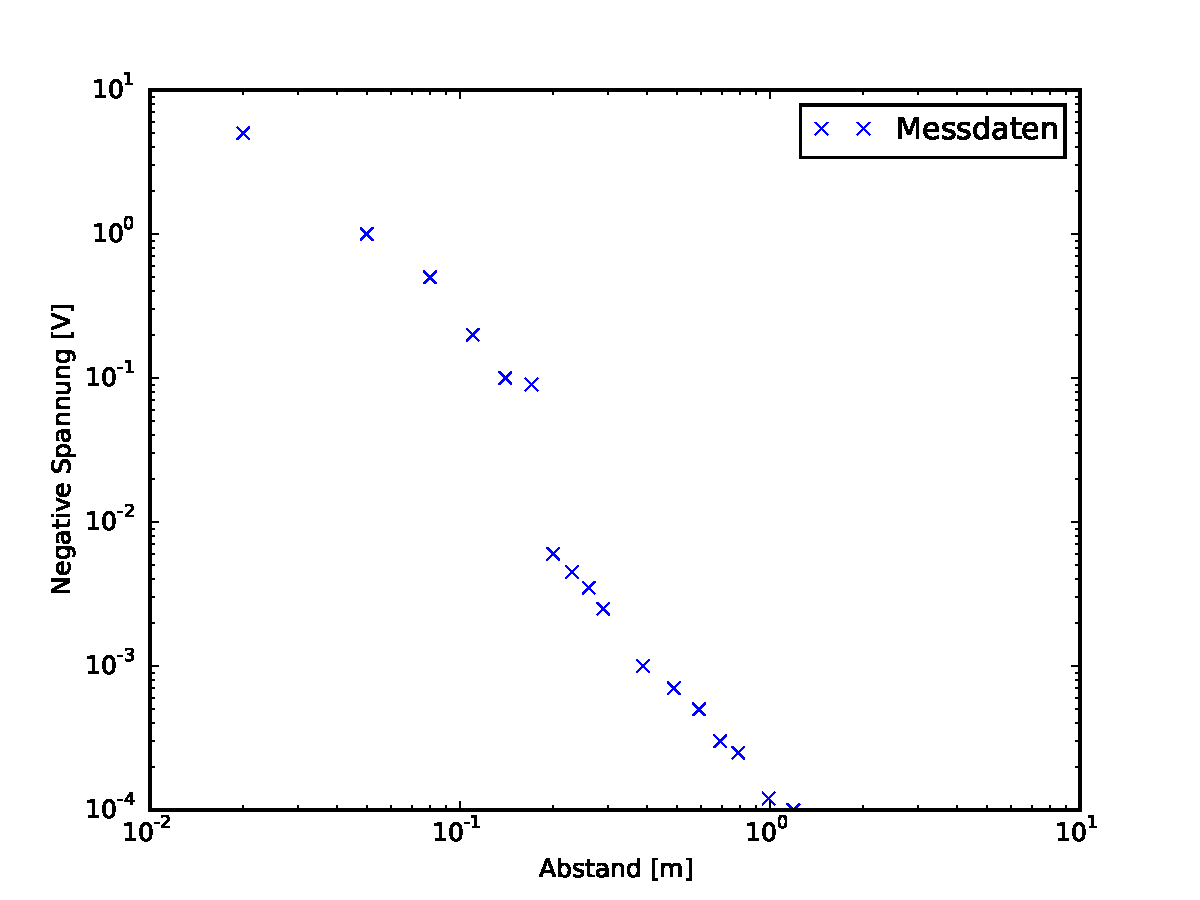
\includegraphics[width=\textwidth]{Bilder/LED_log.pdf}
		\caption{Doppelt-logarithmische Skalierung.}
		\label{diag:LED_log}
	\end{subfigure}
	\caption{Ausgangsspannung des Lock-In-Verstärkers bei Messung mit der LED.}
	\label{diag:LED}
\end{figure}
In \ref{sec:Auswertung1} wurde experimentell nachgewiesen, dass der Betrag der Ausgangsspannung maximal wird, wenn der Phasenschieber auf Vielfache von 180° eingestellt ist.
Bei der Einstellung 0° wird eine maximale, negative Spannung erwartet und den eventuellen Einfluss des Phasenschiebers umgangen.
Das Signal, das von der Photodiode aufgenommen wird, wandelt der Lock-In-Verstärker dementsprechend in eine reine negative Gleichspannung.
Im Interesse der Lesbarkeit werden die negativen Spannung unter Berücksichtigung der Gesamt-Verstärkung in Diagramm \ref{diag:LED} aufgetragen.
Zur Kontrolle, dass die angegebenen Spannungen auf das LED-Signal zurückzuführen sind und nicht von Fremdeinflüssen stammen, wird die LED zeitweise abgedeckt.
Dabei geht bei einem messbaren Signal die Ausgangsspannung auf Null zurück und nimmt ihren ursprünglichen Wert an, wenn der Lichtweg zwischen LED und Photodiode frei gemacht wird.
Der näherungsweise lineare Abfall der Spannung bei doppel-logarithmischer Skalierung \eqref{diag:LED_log} zeigt, dass die gemessene Intensität mit $r^{-\alpha}$ mit $\alpha \in \mathbb{R}$ abfällt.

Bei einem Abstand größer als $\SI{1.20}{\meter}$ ist trotz Verstärkung keine Ausgangsspannung zuverlässig messbar, 
die Ausgangsspannung zeigt beim Abdecken der LED keine wesentliche Änderung.

